% !TEX root = ./paper.tex


% chkTeX linting rules to ignore:
% chktex-file 2   Non-breaking space should have been used.
% chktex-file 3   You should enclose the previous parenthesis with {}
% chktex-file 8   Wrong length of dash may have been used
% chktex-file 21  This command might not be intended
% chktex-file 39  Double space found

%%%%%%%%%%%%%%%%% BODY OF PAPER %%%%%%%%%%%%%%%%%%

\section{Introduction}

In Section~\ref{sec:analysis}, we show this by comparing instantaneous wind torque \(\dot J_\Wind\) of our models to a simple observation-based gyrotrack model based on the work of
The resulting wind torques do however need to be scaled by a factor of \(\sim 7\) in order to yield s presented in Section~\ref{sec:Discussion}.
In Section~\ref{sec:Conclusions} we present our conclusions.



%
% SECTION
%
\section{Analysis}\label{sec:analysis}
\begin{figure}
    \centering
    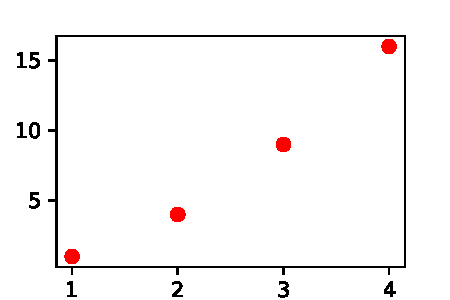
\includegraphics{figures/placeholder.pdf}
    \caption{
        our models.
    }\label{fig:torque}
\end{figure}


% \subsection{Three-dimensional wind models}
In our recent work we have modelled the winds of thirty



%
% SECTION
%
\section{Discussion}\label{sec:Discussion}

Multiple, possibly interacting physical phenomena

%
% SECTION
%
\section{Conclusions}\label{sec:Conclusions}
We have modelled the stellar spin-down rates

\section*{Acknowledgements}
% \begin{enumerate}
    % Funding
    % \item

    % \item
    This project has received funding from the European Research Council (ERC) under the European Union's Horizon 2020 research and innovation programme (grant agreement No 817540, ASTROFLOW).
    % \item
    This work used the Dutch national e-infrastructure with the support of the SURF Cooperative using grant nos. EINF-2218 and EINF-5173.
    % \item
    % We thank SURF (\url{www.surf.nl}) for the support in using the National Supercomputer Snellius.
    % \item
    This research has made use of NASA's \href{https://ui.adsabs.harvard.edu/}{Astrophysics Data System}.
    % Software
    % \item
    This work was carried out using the \swmf{} tools developed at The University of Michigan \href{https://spaceweather.engin.umich.edu/the-center-for-space-environment-modelling-csem/}{Center for Space Environment Modelling (CSEM)} and made available through the NASA \href{https://ccmc.gsfc.nasa.gov/}{Community Coordinated Modelling Center (CCMC)}.
    % \item
    This work has made use of the following additional numerical software, statistics software and visualisation software:
          NumPy~\citep{2011CSE....13b..22V},
          SciPy~\citep{2020SciPy-NMeth},
     Matplotlib~\citep{2007CSE.....9...90H},
     and
    statsmodels~\citep{seabold2010statsmodels}.
    % \item
    %We would like to express our gratitude to the anonymous reviewers for their valuable contributions, which have enhanced the quality and rigour of our article.
% \end{enumerate}

\section*{Data availability}
The data underlying this article will be shared on reasonable request to the corresponding author.

%%%%%%%%%%%%%%%%%%%%%%%%%%%%%%%%%%%%%%%%%%%%%%%%%%